%----------------------------------------------------------------------------------------
%
% A LaTeX-template for 1DV510. Modified and translated by Björn Lindenberg at LNU.
% Based on an original master thesis template created by Marcus Wilhelmsson at LNU.
%
%----------------------------------------------------------------------------------------

% Settings and document configuration

\documentclass[a4paper,12pt]{article} 
\usepackage[T1]{fontenc} 
\usepackage{times} 
\usepackage[swedish,english]{babel} 
\usepackage[utf8]{inputenc} 
\usepackage{dtk-logos} 
\usepackage{wallpaper} 
\usepackage[absolute]{textpos} 
\usepackage[top=2cm, bottom=2.5cm, left=3cm, right=3cm]{geometry} 
\usepackage[parfill]{parskip} 
\usepackage{csquotes} 
\usepackage{float} 
\usepackage{lipsum} % Used for dummy text. Can be removed.
\usepackage{listings, color}
\lstdefinestyle{Asm}{
  belowcaptionskip=1\baselineskip,
  breaklines=true,
  frame=L,
  xleftmargin=\parindent,
  language=[x86masm]Assembler,
  showstringspaces=false,
  basicstyle=\footnotesize\ttfamily,
  keywordstyle=\bfseries\color{purple!40!black},
  commentstyle=\itshape\color{green!40!black},
  identifierstyle=\color{blue},
  stringstyle=\color{orange},
}

% Fontsizes for section headings.
\usepackage{sectsty} 
\sectionfont{\fontsize{14}{15}\selectfont}
\subsectionfont{\fontsize{12}{15}\selectfont}
\subsubsectionfont{\fontsize{12}{15}\selectfont}

%----------------------------------------------------------------------------------------
%	This part is used for the text box on the title page
%----------------------------------------------------------------------------------------
\newsavebox{\mybox}
\newlength{\mydepth}
\newlength{\myheight}

\newenvironment{sidebar}%
{\begin{lrbox}{\mybox}\begin{minipage}{\textwidth}}%
{\end{minipage}\end{lrbox}%
 \settodepth{\mydepth}{\usebox{\mybox}}%
 \settoheight{\myheight}{\usebox{\mybox}}%
 \addtolength{\myheight}{\mydepth}%
 \noindent\makebox[0pt]{\hspace{-20pt}\rule[-\mydepth]{1pt}{\myheight}}%
 \usebox{\mybox}}

%----------------------------------------------------------------------------------------
%	Title
%----------------------------------------------------------------------------------------
\newcommand\BackgroundPic{
    \put(-2,-3){
    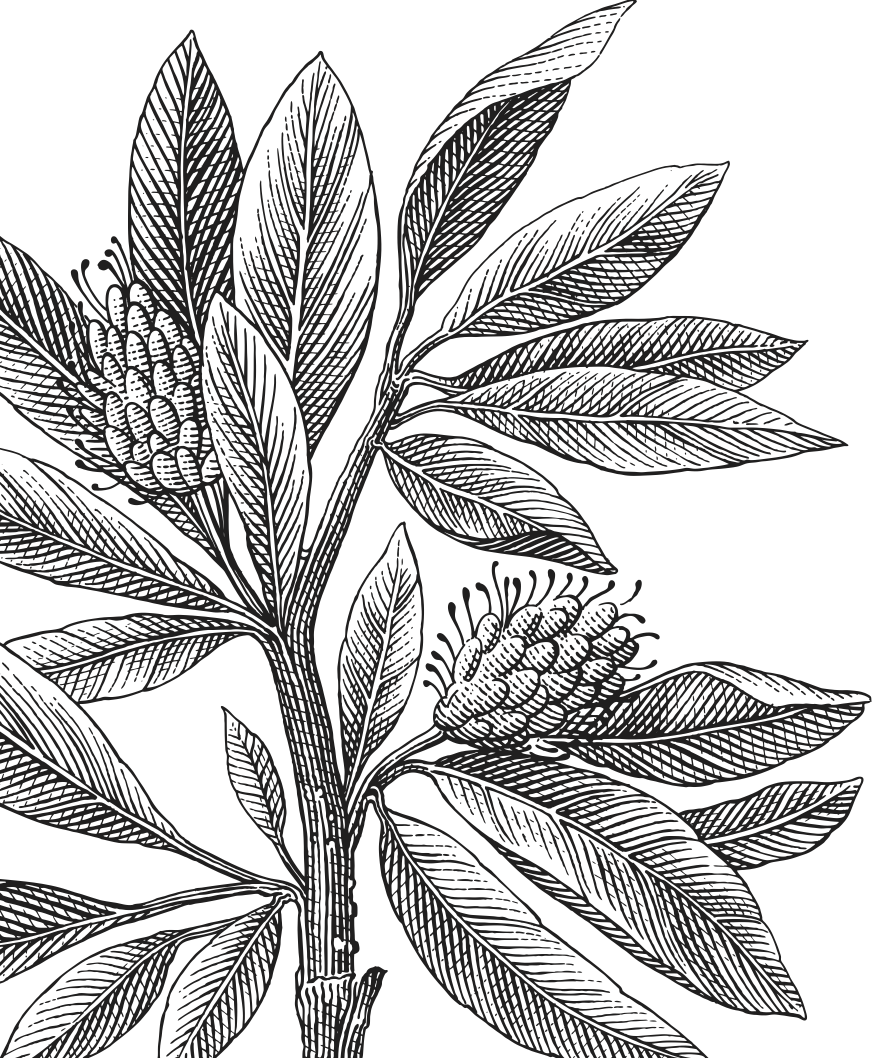
\includegraphics[keepaspectratio,scale=0.3]{img/lnu_etch.png} % Background image
    }
}
\newcommand\BackgroundPicLogo{
    \put(30,740){
    
\includegraphics[keepaspectratio,scale=0.10]{img/logo.png} % LNU logo
    }
}

\title{
\vspace{-8cm}
\begin{sidebar}
    \vspace{10cm}
    \normalfont \normalsize
    \huge Computer Technology I\\ % Main title
    \vspace{-1.3cm}
\end{sidebar}
\vspace{3cm}
\begin{flushleft}
    \huge Lab. 1 : How to use the PORTs, Digital input/output, Subroutine call % Subtitle
     \small \\ \emph{}
\end{flushleft}
\null
\vfill
\begin{textblock}{5}(10,13)
\begin{flushright}
\begin{minipage}{\textwidth}
\begin{flushleft} \large
\emph{Author:}\textsc{}\\  % Author
\emph{Supervisor:}  \textsc{} \\  % Author
\emph{Semester:} Autumn 2019\\ % Semester
\emph{Area:} Computer Science \\ % Area
\emph{Course code:} 1DT301 % Course
\end{flushleft}
\end{minipage}
\end{flushright}
\end{textblock}
}

\date{} % Empty date command. Use \today inside for today's date.
\author{} % Normally one would use this to define authors. However in this case the title command takes care of everything, so we leave the field empty to get rid of warnings. 

\begin{document}

\pagenumbering{gobble} % Turn off page numbering
\newgeometry{left=5cm}
\AddToShipoutPicture*{\BackgroundPic} % Adds the background image to the title page
\AddToShipoutPicture*{\BackgroundPicLogo} % Adds the logo to the title page
\maketitle % Prints the title
\restoregeometry
\clearpage

\pagenumbering{roman} % Roman page numbering for abstract page


\selectlanguage{english}

\newpage

\pagenumbering{gobble} % Turn off page numbering
\tableofcontents 

\newpage
\pagenumbering{arabic} % Turn on page numbering


\section{Task 1}
For the first task the goal was to get a light blinking. This was done by setting the data direction register to output, and after that setting the LED port low.

\lstset{style=Asm}

\begin{lstlisting}
;>>>>>>>>>>>>>>>>>>>>>>>>>>>>>>>>>>>>>>>>>>
;	1DT301, Computer Technology 1
;	Date: 09-09-2019
;	Authors:
;		Roel de Vries
;		Anas Kwefati
;
;	Lab number 1
;	Title:	How to use the PORTS, digital IO, subroutine call
;
;	Hardware: STK600, CPU ATmega 2560
;
;	Function: Turn on LED 2
;
;	Input ports: None
;
;	Output ports: PORTB, used for LEDS
;
;	Subroutines: None
;	Included files: m2560def.inc
;
;	Other information: None
;
;	Changes in program: 
;		09-09-2019 > file created
;<<<<<<<<<<<<<<<<<<<<<<<<<<<<<<<<<<<<<<<<<<
.include "m2560def.inc"

main: 
	SBI DDRB, 2
	CBI PORTB, 2
	
\end{lstlisting}
Here is the flowchart : 

\begin{figure}
\begin{center}
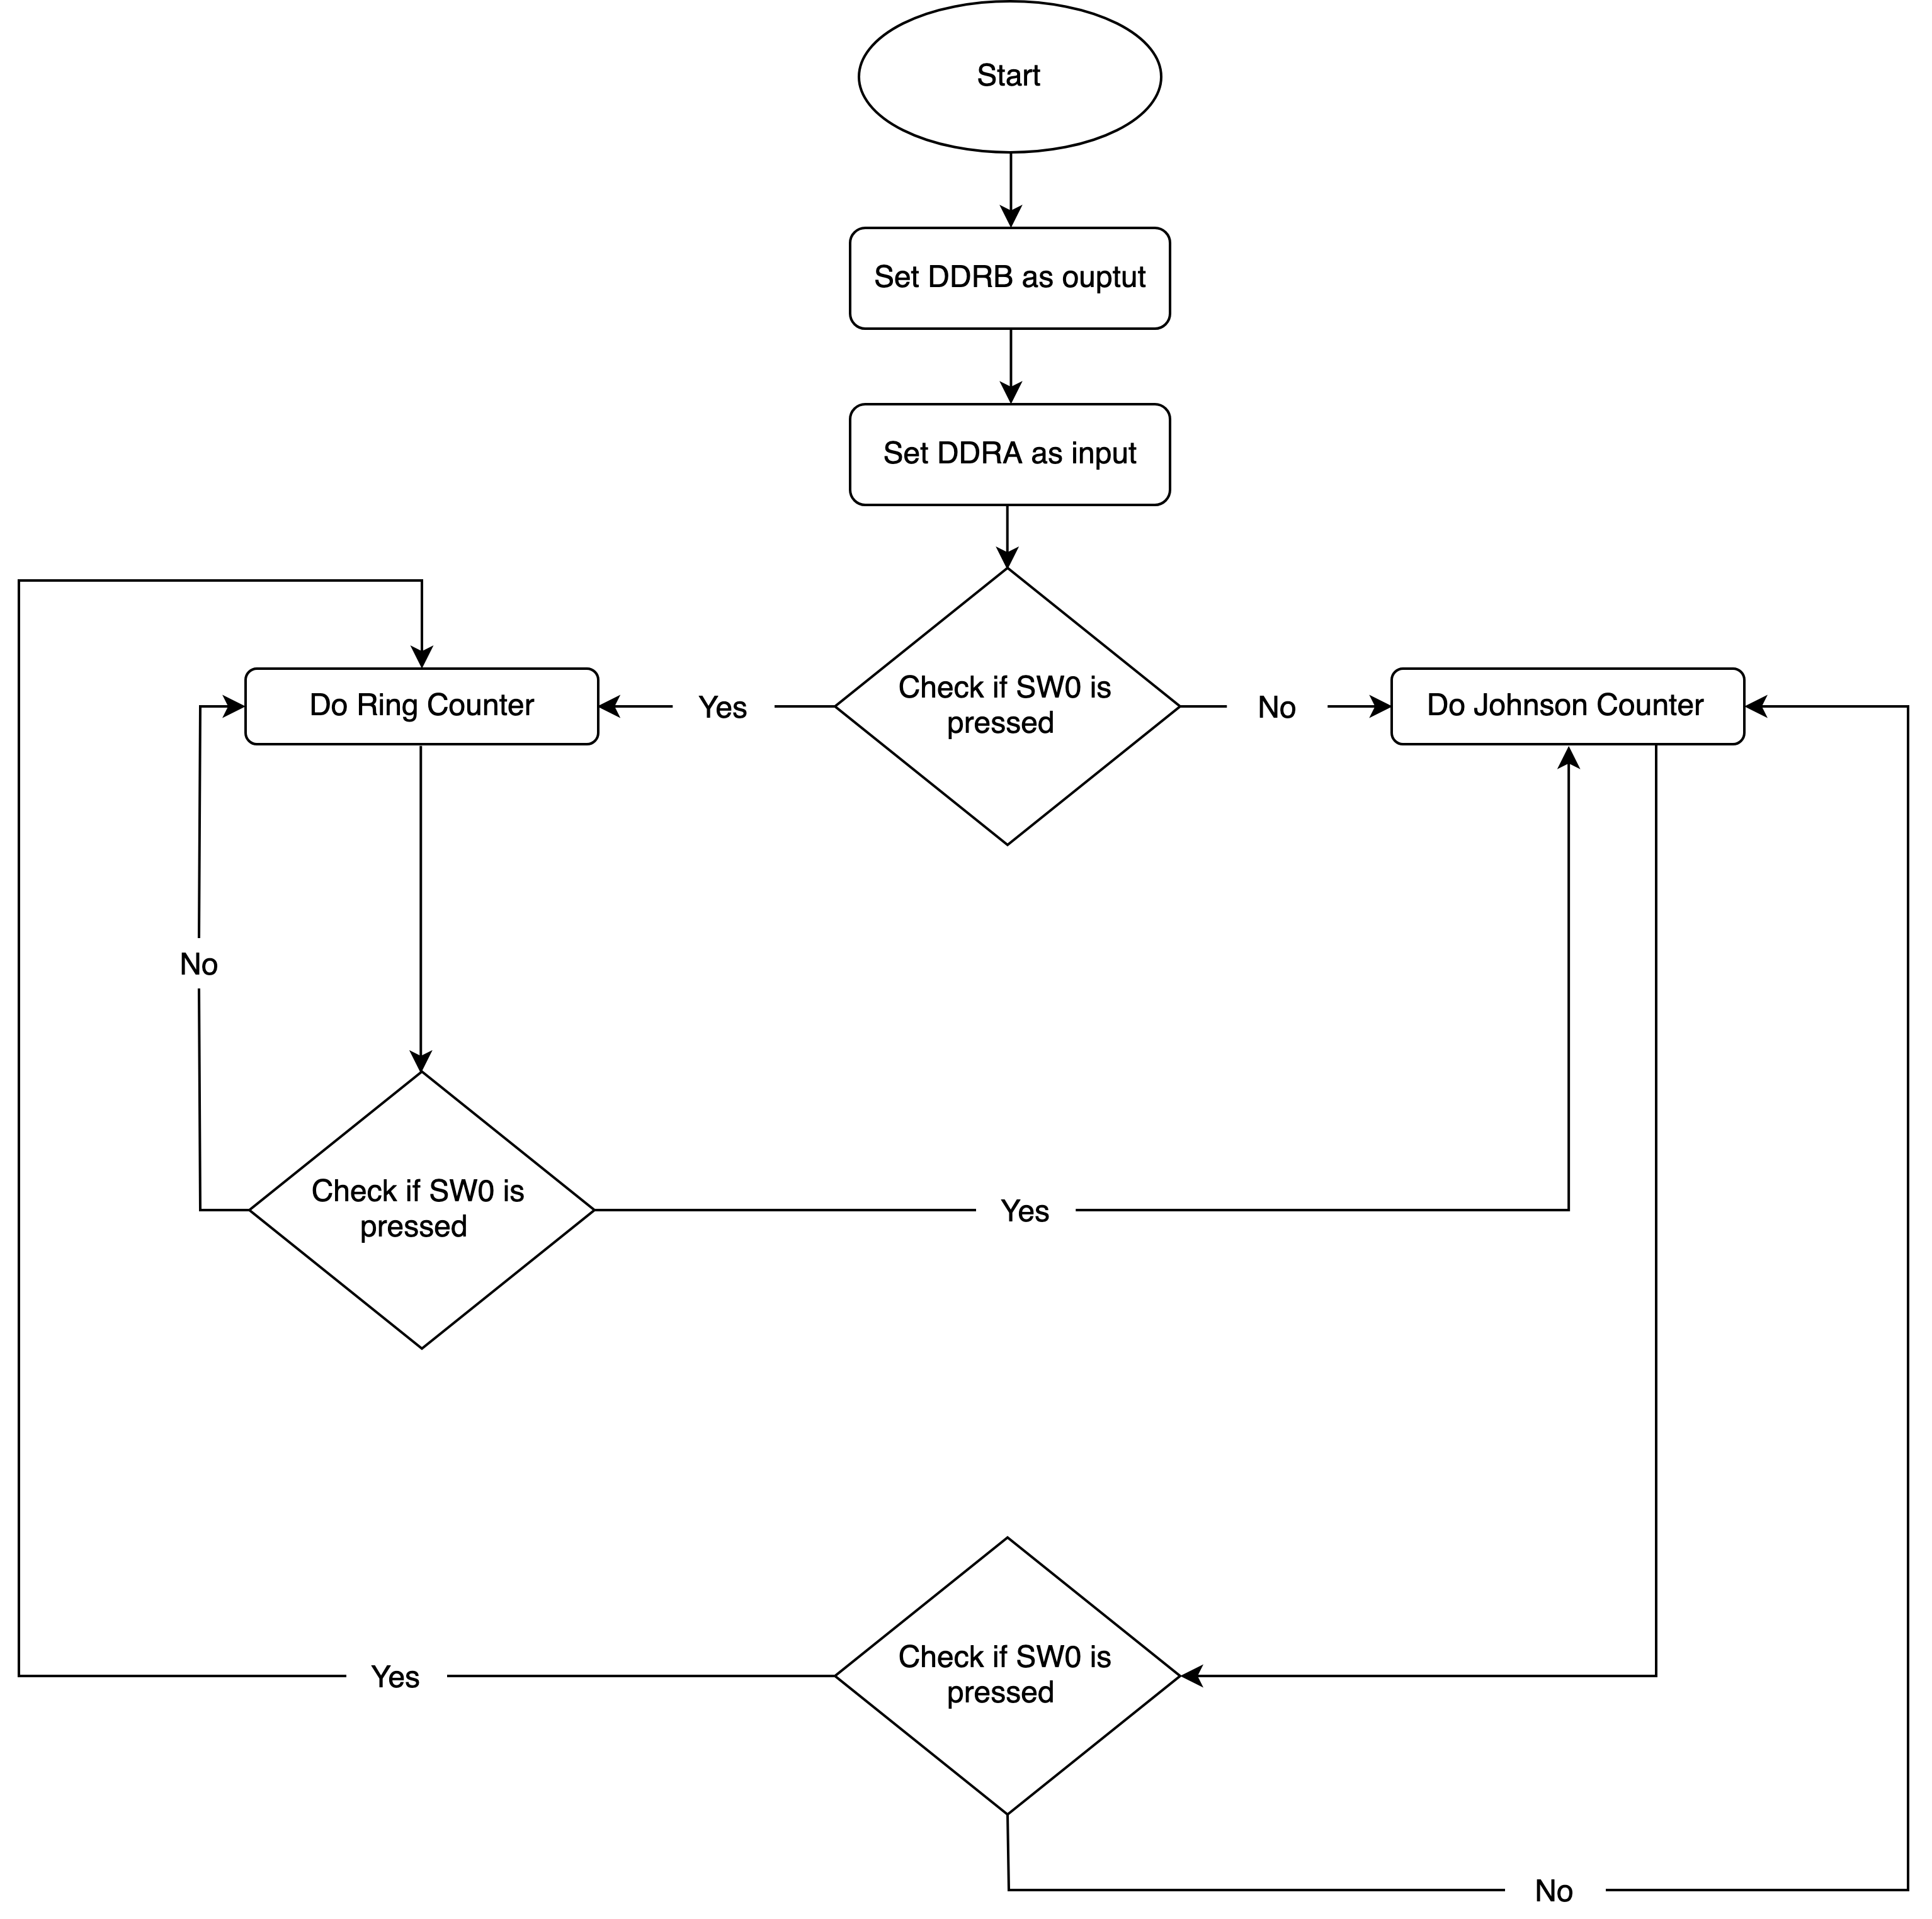
\includegraphics[width = 6cm, height=8cm]{flowchart/task1_flowchart.PNG}
\end{center}
\caption{Task 1 flowchart}
\label{task1}
\end{figure}
\break



%TASK2
\section{Task 2}
For the second task the aim is to read switches and light to corresponding LED. This was done by using a data direction register 
\lstset{style=Asm}

\begin{lstlisting}
;>>>>>>>>>>>>>>>>>>>>>>>>>>>>>>>>>>>>>>>>>>>>>>>>>>>>>>>>>>>
; 1DT301, Computer Technology I
; Date: 2019-09-95
; Author:
;   Roel de Vries
;   Anas Kwefati
;
;	Lab number 1
;	Title:	How to use the PORTS, digital IO, subroutine call
;
;	Hardware: STK600, CPU ATmega 2560
;
;	Function: Turn on Led n if switch n is pressed
;
;	Input ports: PORTA, used for the switches
;
;	Output ports: PORTB, used for LEDS
;
;	Subroutines: None
;	Included files: m2560def.inc
;
;	Other information: None
;
;	Changes in program:
;		09-09-2019 > file created
;
;<<<<<<<<<<<<<<<<<<<<<<<<<<<<<<<<<<<<<<<<<<<<<<<<<<<<<<<<<<<



;TASK_2

;Load pre-configured files for the ports and memory adresses
.include "m2560def.inc"

ldi r16, 0xFF ; load 0b1111 1111 to r16
out DDRB, r16 ; we set the Data Direction Register B to be ready to give an output to turn on the light (0 is on and 1 is off) so now we are outputting 1

ldi r17, 0x00 ; we load 0b0000 0000 to the register 17
out DDRD, r17 ; we set the Data Direction Register D to take an input  

ldi r16, 0xFF ; 
out PORTB, r16 ; we are setting the PORTB to give an output of 0b1111 1111 like that the light is off (for LED 0 is on and 1 is off) 

; we are creating an infinite loop to check if the switch port is on or off
infinite_loop_switch:

	in r18, PIND ; The input data received from the input PIND is stored in the register r18
	out PORTB, r18 ;The PORTB will take the data of r18 and output it to the LED and turn on the light if it is correct 

rjmp infinite_loop_switch ;we repeat the process


\end{lstlisting}

Here is the flowchart for this task : 
\begin{figure}
\begin{center}
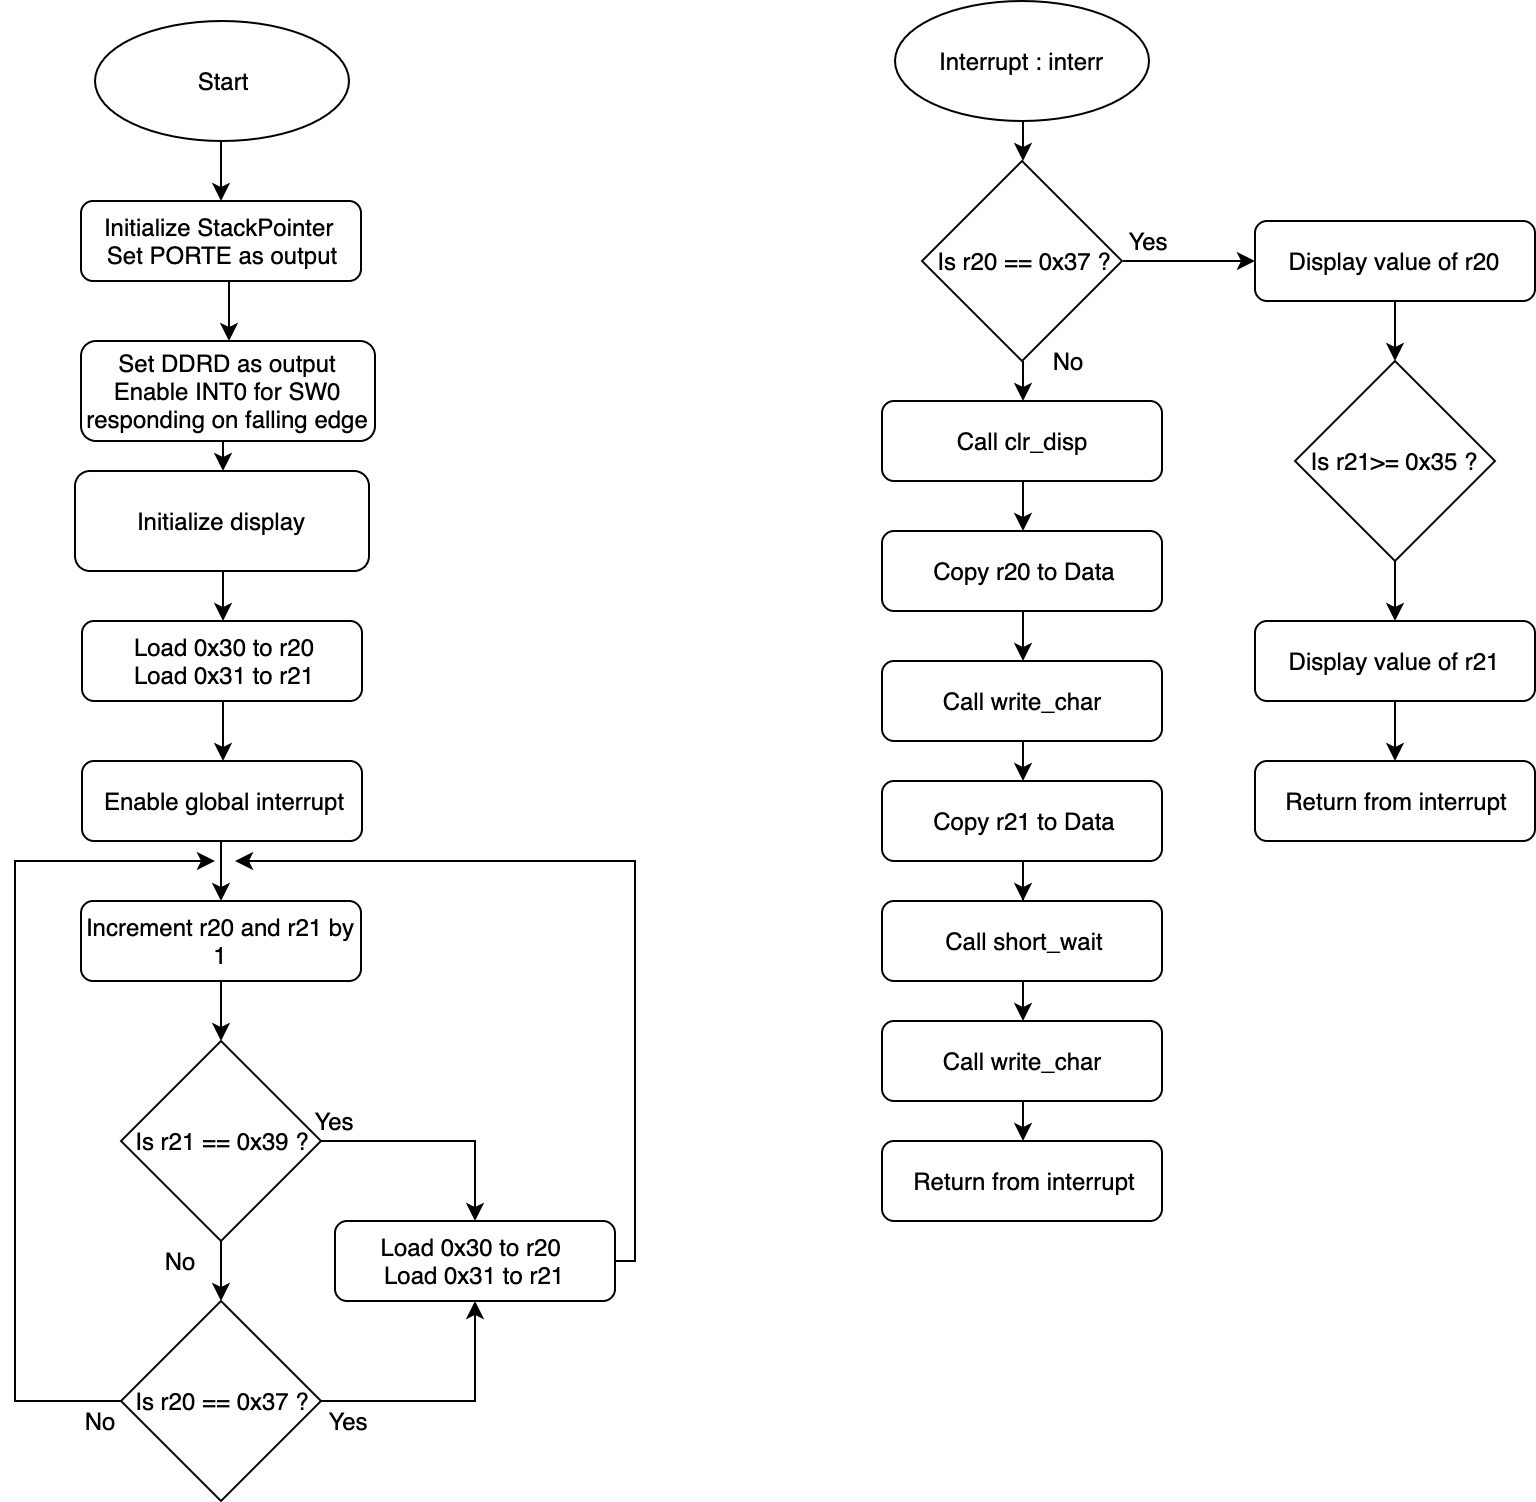
\includegraphics[width = 6cm, height=14cm]{flowchart/task2_flowchart.PNG}
\end{center}
\caption{Task 2 flowchart}
\label{task2}
\end{figure}

\break

\section{Task 3}
In task 3 the goal was to turn on led 0, only if switch 5 was pressed. by checking if the bit for switch 5 is high we are able to turn the led on at the right moment

\lstset{style=Asm}

\begin{lstlisting}
;>>>>>>>>>>>>>>>>>>>>>>>>>>>>>>>>>>>>>>>>>>
;	1DT301, Computer Technology 1
;	Date: 09-09-2019
;	Authors:
;		Roel de Vries
;		Anas Kwefati
;
;	Lab number 1
;	Title:	How to use the PORTS, digital IO, subroutine call
;
;	Hardware: STK600, CPU ATmega 2560
;
;	Function: Turn on Led 0 when you press led 5
;
;	Input ports: PORTA, used for the switches
;
;	Output ports: PORTB, used for LEDS
;
;	Subroutines: None
;	Included files: m2560def.inc
;
;	Other information: None
;
;	Changes in program: 
;		09-09-2019 > file created
;<<<<<<<<<<<<<<<<<<<<<<<<<<<<<<<<<<<<<<<<<<
.include "m2560def.inc"

main:
	SBI DDRB, 0 ; set output
	CBI DDRA, 5 ; set input

lightloop:

	SBIS PINA, 5
	CBI PORTB, 0
	SBIC PINA, 5	
	SBI PORTB, 0  
\end{lstlisting}

\section{Task 4}
In task 4 we needed to run the task 3 code in the simulator, as seen in the screenshots below, this worked.

TBD

\section{Task 5}
For task 5 we needed to create a ring counter. This was done by creating a loop which constantly shifts the PORTB register one sideways with a delay.

\lstset{style=Asm}

\begin{lstlisting}
;>>>>>>>>>>>>>>>>>>>>>>>>>>>>>>>>>>>>>>>>>>
;	1DT301, Computer Technology 1
;	Date: 09-09-2019
;	Authors:
;		Roel de Vries
;		Anas Kwefati
;
;	Lab number 1
;	Title:	How to use the PORTS, digital IO, subroutine call
;
;	Hardware: STK600, CPU ATmega 2560
;
;	Function: Creates a ring counter, updates every 0.5 seconds
;
;	Input ports: None
;
;	Output ports: PORTB, used for LEDS
;
;	Subroutines: Timer
;	Included files: m2560def.inc
;
;	Other information: None
;
;	Changes in program: 
;		09-09-2019 > file created
;<<<<<<<<<<<<<<<<<<<<<<<<<<<<<<<<<<<<<<<<<<
.include "m2560def.inc"

main:
	; Initialize SP, Stack Pointer
	ldi r20, HIGH(RAMEND) ; R20 = high part of RAMEND address
	out SPH,R20 ; SPH = high part of RAMEND address
	ldi R20, low(RAMEND) ; R20 = low part of RAMEND address
	out SPL,R20 ; SPL = low part of RAMEND address

	LDI r20, 0xFF
	OUT DDRB, r20
	CBR r20, 1 ; set output
	OUT PORTB, r20
	call timer

lightloop:
	LSL r20
	BRCS setbit
lightloopcont:
	OUT PORTB, r20
	call timer
	call lightloop

setbit:
	SBR r20, 1
	CLC
	call lightloopcont

timer:
; Generated by delay loop calculator
; at http://www.bretmulvey.com/avrdelay.html
	ldi  r17, 5
    ldi  r18, 20
    ldi  r19, 175
L1: dec  r19
    brne L1
    dec  r18
    brne L1
    dec  r17
    brne L1
	ret

\end{lstlisting}

\section{Task 6}
The Johnson counter was created by using two smaller loops who constantly call eachother. the first which increases the amount of leds on, and a second which decreases the amount of leds on.

\lstset{style=Asm}

\begin{lstlisting}
;>>>>>>>>>>>>>>>>>>>>>>>>>>>>>>>>>>>>>>>>>>
;	1DT301, Computer Technology 1
;	Date: 09-09-2019
;	Authors:
;		Roel de Vries
;		Anas Kwefati
;
;	Lab number 1
;	Title:	How to use the PORTS, digital IO, subroutine call
;
;	Hardware: STK600, CPU ATmega 2560
;
;	Function: Creates a johnson counter, updates every 0.5 seconds
;
;	Input ports: None
;
;	Output ports: PORTB, used for LEDS
;
;	Subroutines: Timer
;	Included files: m2560def.inc
;
;	Other information: None
;
;	Changes in program: 
;		09-09-2019 > file created
;<<<<<<<<<<<<<<<<<<<<<<<<<<<<<<<<<<<<<<<<<<
.include "m2560def.inc"

main:
	; Initialize SP, Stack Pointer
	ldi r21, HIGH(RAMEND) ; R20 = high part of RAMEND address
	out SPH,R21 ; SPH = high part of RAMEND address
	ldi R21, low(RAMEND) ; R20 = low part of RAMEND address
	out SPL,R21 ; SPL = low part of RAMEND address

	CBR r16, 0; counter
	SBR r17, 255; light state 
	OUT DDRB, r17
	ldi r16, 8

incloop:
	LSL r17
	OUT PORTB, r17
	call timer
	dec r16
    brne incloop
	ldi r16, 8
	call decloop

decloop:
	LSR r17
	SBR r17, 128
	OUT PORTB, r17
	call timer
	dec r16
    brne decloop
	ldi r16, 8
	call incloop

timer:
; Generated by delay loop calculator
; at http://www.bretmulvey.com/avrdelay.html
	ldi  r18, 5
    ldi  r19, 20
    ldi  r20, 175
L1: dec  r20
    brne L1
    dec  r19
    brne L1
    dec  r18
    brne L1
    rjmp PC+1
	ret

\end{lstlisting}


% Prints your bibliography database xxx.bib
\bibliographystyle{IEEEtran}
\bibliography{ref.bib}

\end{document}
